\section{Kürzeste Wege Probleme}
\begin{definition}[gewichteter Graph]
Sei $G=(V,E)$ ein Graph. Eine \emph{Gewichtsfunktion} für die Kanten von $G$ ist eine Abbildung $w \colon E \to R$. Ist $\pi=v_0,v_1,\ldots,v_r$ ein Weg, so heißt
\[
w(\pi) = \sum_{i=1}^{r-1}w(v_i,v_{i+1})
\]
die \emph{Weglänge} von $\pi$ bezüglich $w$. Das Trippel $G=(V,E,w)$ heißt \emph{gewichteter Graph}. 
\end{definition}
\begin{definition}
	\label{def:negative_gewichte}
Sei $G=(V,E,w)$  ein gewichteter Graph und $v, \tilde{w} \in  V$. Ein \emph{kürzester Weg} von $v$ nach $\tilde{w}$  in $G$  bezüglich $w$ ist ein $v\text{-} \tilde{w}$-Weg $\pi$  mit der Eigenschaft $w(\pi) \le w(\pi')$  für alle anderen $v\text{-}w$-Wege $\pi'$ .
Die kürzeste Weglänge $\delta(v,\tilde{w})$  von $v$ nach $\tilde{w}$ ist definiert durch:

\begin{center}$\delta(v,\tilde{w}) \begin{cases}
	\min \{w(\pi) | \pi \text{ ist $v$-$\tilde{w}$-Weg  }\} &, \text{falls ein solcher Weg existiert} \\
	\infty &, \text{ sonst}
\end{cases}$ \end{center}
\end{definition}

\begin{example}
Betrachte den gewichteten Graph $G=(V,E,w)$ mit

\begin{center}
\begin{tikzpicture}

%Nicer Graph


\end{tikzpicture}
\end{center}
Mögliche Wege von $v_3$ nach $v_1$ sind:
\begin{align*}
	\pi_1&=v_3,v_1 &\implies w(\pi_1)&=6 \\
	\pi_2&=v_3,v_2,v_1 &\implies w(\pi_2)&=5 \\
	\pi_3&=v_3,v_4,v_2,v_1 &\implies w(\pi_3)&=9
\end{align*}
\end{example}
\begin{notation}
Wir werden im Folgenden nur Digraphen behandeln, da sich ungerichtete Graphen immer auch als gerichtete Graphen interpretieren lassen.
Sei $G=(V,E,w) $ ein gewichteter Digraph.
\end{notation}
Wir unterscheiden drei verschiedene Varianten des \emph{kürzeste-Wege-Problems:}
\begin{enumerate}
	\item Einzelpaar-kürzeste-Wege-Problem \\
		Gegeben $v,u \in V$ , suche einen kürzesten Weg von v nach u.
	\item Einzelquelle-kürzeste-Wege-Problem \\
		Gegeben $v \in V$, suche einen kürzesten Weg von $v$ zu allen $u \in post^{*}(v)$.  
	\item Alle-Paare-kürzeste-Wege-Problem \\
		Finde alle Paare $v,u \in V$ einen kürzesten $v$-$u$-Weg
\end{enumerate}
Wir bemerken, dass das Problem c die Probleme a und b löst, daher betrachten wir im Folgenden nur Problem c. \\
Negative Gewichte sind zwar nach Definition \ref{def:negative_gewichte} zugelassen, können aber Probleme bereiten:
\begin{example}
Betrachte:
\begin{center}
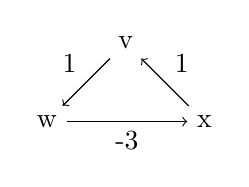
\begin{tikzpicture}
 \node (v) at (0,0) {v};
 \node (w) at (-1,-1) {w};
 \node (x) at (1,-1) {x};

 \path [->] (v) edge node[above left] {1} (w);
 \path [->] (w) edge node[below] {-3} (x);
 \path [->] (x) edge node[above right] {1} (v);
\end{tikzpicture}
\end{center}
In diesem Graphen gibt es keinen kürzesten Weg.
\begin{align*}
	w(v,w,x)&=-2 \\
	w(v,w,x,v,w,x)&=-3
\end{align*}
Man kann den Weg also immer weiter verlängern und der Weg wird immer kürzer.
\end{example}
\begin{lemma}
	Sei $G=(V,E,w)$  ein gewichteter Digraph. Falls es in $G$ keine Zyklen mit negativer Weglänge gibt, dann gibt es für $v,u \in V, u \in  post^{*}(v)$ einen kürzesten Weg $\pi$ mit:
	\[
	\delta(v,w) = w(\pi) > -\infty
	\]
\end{lemma}
\begin{proof}
Da es keine negativen Zyklen gibt, genügt es alle einfachen Wege von $v$ nach $u$ zu betrachten. Da $|V|$ und $|E|$ endlich sind, sind dies endlich viele, so dass $\pi$ durch einen Minimierer gegeben ist.
\end{proof}

\begin{lemma}
	\label{lem:teilweg}
	Sei $G=(V,E,w)$ ein gewichteter Digraph ohne negativen Zyklen. Ist $\pi= v_0, \ldots, v_r$ ein kürzester Weg von $v_0$  nach $v_r$ dann ist der Teilweg
	\[
		\pi_{i,j} =v_i,\ldots,v_j, 0\le i  <j \le r
	\]
ein kürzester Weg von $v_i$ nach $v_j$.
\end{lemma}
\begin{proof}
\underline{Angenommen:} $\pi_{i,j}'$ ist ein kürzester Weg von $v_i$ nach $v_j$ mit $w(\pi_{i,j}'  < w (\pi_{i,j})$
\begin{align*}
	\implies \pi' &= \pi_{0,i} \pi_{i,j}' \pi_{j,r} \text{ erfüllt:}\\
	w(\pi')&= w(\pi_{0,i})+w(\pi_{i,j}')+w(\pi_{j,r}) \\
	       &< w(\pi_{0,i})+ w(\pi_{i,j} + w(\pi_{j,r})\\
	       &= w(\pi') \\
	       &\implies w(\pi') < w(\pi)
\end{align*}
Dies ist ein Widerspruch, da $\pi$ kürzester Weg nach Annahme ist.
\end{proof}
\begin{lemma}
	Sei $G=(V,E,w)$ ein gewichteter Digraph ohne negative Zyklen und sei $\pi=v_0,v_1,\ldots,v_r$ ein kürzester Weg von $v_0$ nach $v_r$ . Dann gilt:
	\[
	\delta(v_0,v_r)= \delta(v_0, v_{r-1} + w(v_{r-1}, v_r)
	\]
\end{lemma}
\begin{proof}
Aus Lemma \ref{lem:teilweg} folgt:
\begin{itemize}
	\item $\pi' = v_0,\ldots, v_{r-1}$ ist ein kürzester Weg von $v_0$ nach $v_{r-1}$
	\item $\delta(v_0,v_{r-1} = w(\pi')$
	\item $\delta(v_0,v_r)= w(\pi)$	
\end{itemize}
$w(\pi)$ lässt sich umschreiben:
\begin{align*}
	w(\pi)&= w(\pi')+w(v_{r-1},v_r) \\
	      &= \delta(v_0,v_{r-1} + w(v_{r-1},v_r)
\end{align*}
\end{proof}

\begin{algorithm}[H]
	\label{alg:dijkstra}
	\caption{Dijkstra Algorithmus}
	\KwData{Gewichteter Graph $G=(V,E,w)$ mit nicht negativen Gewichten}
	\KwResult{Kürzeste Wege von $s$ nach $v \in post^{*}(s)$ samt Weglänge $l(v)=\delta(s,v)$}
\begin{itemize}
	\item $l(s)=0$ \\$l(v) = \infty$, $v \in V \setminus \{s\} $ \\$R=\emptyset$ 
	\item Finde $u \in V\setminus R$ mit $l(n)= \min_{v \in V \setminus R} l(v)$
	\item $R=R \cup \{u\} $ 
	\item \For{$v \in V \setminus R$ mit $(u,v) \in E$}{
			\If{$l(v)> l(u)+w(u,v)$}{
				$l(v) = l(u)+w(u,v)$\\
				$p(v)=u$ }}
	\item $R \neq  V $ gehe zu 2. 
\end{itemize}
\end{algorithm}
\begin{remark}
Die kürzesten Wege im Output des Algorithmus sind durch die Abbildung $p \colon V \to V $ gegeben, denn
\[
	\pi=s,\ldots, p(p(p(v))),p(p(v)),p(v),v
\]
ist ein kürzester $s$-$v$-Weg.
\end{remark}
\begin{example}
Der Graph
\begin{center}
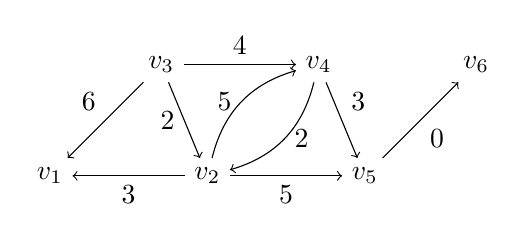
\begin{tikzpicture}[node distance = 2cm, auto]

	\node (v3) {$v_3$};
	\node (v4) [right of=v3] {$v_4$};
	\node (v1) [below left of=v3] {$v_1$};
	\node (v2) [right of=v1] {$v_2$};
	\node (v5) [right of=v2] {$v_5$};
	\node (v6) [above right of=v5] {$v_6$};

	\path[->] (v5) edge node[below right] {0} (v6);
	\path[->] (v2) edge node[below] {5} (v5);
	\path[->] (v2) edge node[below] {3} (v1);
	\path[->] (v4) edge node[above right]{3} (v5);
	\path[->] (v3) edge node[above left] {6} (v1);
	\path[->] (v3) edge node[above] {4} (v4);
	\path[->] (v4) edge[bend right=-30] node[right] {2} (v2);
	\path[->] (v2) edge[bend left=30] node[left] {5} (v4);
	\path[->] (v3) edge node[left] {2} (v2);
		
\end{tikzpicture}
\end{center}
mit Startknoten $v_3$ hat nach Ausführung von Algorithmus \ref{alg:dijkstra} folgende Ausgabe:
\clearpage
\begin{table}[htbp]
	\centering\renewcommand{\arraystretch}{1.2}
	\caption{Dijkstra}
	\label{tab:dijkstra}
	\begin{tabular}{c|c c c c c c| c c c}
Iteration & \multicolumn{6}{c|}{$l(v_1),l(v_2),\ldots,l(v_6)$} & \multicolumn{3}{c}{$u$, $l(u)$, $p(u)$  } \\
\hline
$0$ & $\infty$ & $\infty$ & $0$ & $\infty$ & $\infty$ & $\infty$ & $v_3$ & $0$ &$-$ \\     
$1$ & $6$ & $2$ & & $4$ & $\infty$ & $\infty$ & $v_2$ & $2$ & $v_3$ \\
$2$ & $5$  & & & &  $7$ & $\infty$ & $v_4$ & $4$ & $v_3$  \\
$3$ & & & & & & $\infty$ & $v_1$ & $5$ & $v_2$ \\
$4$ & & & & & & $\infty$ & $v_5$ & $7$ & $v_2$ \\
$5$ & & & & & & $7$ & $v_6$ & $7$ & $v_5$ \\
	\end{tabular}
\end{table}
\end{example}
\begin{theorem}
Der Algorithmus von Dijkstra \ref{alg:dijkstra} arbeitet korrekt, mit einer Laufzeit von $\mathcal{O}(n^2), n=|V|$.
\end{theorem}


